% !TeX spellcheck = en_US
\documentclass[
	english,
	openany,
	draft = false,
	twoside = true,
	fleqn
]{scrbook}
\usepackage{learning-notes}

\author{Huu Duc Nguyen}
\authordegreefront{}
\authordegreeback{ M.Sc.}
\subject{Robotics}
\title{Robotics Notes}
\date{07 May 2022}

\begin{document}
	\setlength{\abovedisplayskip}{3pt}
	\setlength{\belowdisplayskip}{3pt}
	
	\frontmatter
	\TitlePage
	\tableofcontents
	
	\mainmatter
	% !TeX spellcheck = en_GB
\chapter*{Abbreviations}
\addcontentsline{toc}{chapter}{Abbreviations}

\begin{acronym}[LONGEST]
\acro{AI}{Artificial Intelligence}
\acro{AGI}{Artificial General Intelligence}
\acro{ML}{Machine Learning}
\acro{DL}{Deep Learning}
\acro{CS}{Computer Science}
\acro{CV}{Computer Vision}
\acro{RL}{Reinforcement Learning}
\acro{NLP}{Natural Language Processing}
\acro{GPU}{Graphics Processing Unit}
\acro{CPU}{Central Processing Unit}

% Conferences
\acro{ICML}{\href{https://icml.cc/}{International Conference on Machine Learning}}

\acro{prob}[prob.]{probability}
\acro{param}[params.]{parameters}
\acro{algor}[algor.]{algorithms}
\acro{info}[info.]{information}
\acro{aka}[a.k.a.]{also known as}
\acro{wrt}[w.r.t.]{with regard to}
\acro{no}[no.]{number of}
\acro{func}[func.]{function}
\acro{vs}[vs.]{versus}
\acro{freq}[freq.]{frequency}
\acro{st}[s.t.]{subject to}

\acro{iid}[i.i.d.]{independent \& identically distributed}
\acro{LSI}{linear shift invariant}
\acro{pdf}[pdf.]{Probability Density Function}
\acro{MLE}{Maximum Likelihood Estimation}
\acro{MAP}{Maximum A Posteriori}
\acro{MoG}{Mixture of Gaussians}
\acro{SVM}{State Vector Machine}

% Gradient descent
\acro{GD}{Gradient Descent}
\acro{SGD}{Stochastic Gradient Descent}
\acro{nag}[NAG]{Nestorov Accelerated Gradient}
\acro{rmsprop}[RMSprop]{Root mean squared prop}
\acro{adam}[Adam]{Adaptive moment estimation}

\acro{SVD}{Singular Value Decomposition}
\acro{PCA}{Principal Component Analysis}
\acro{LDA}{Linear Discriminant Analysis}
\acro{KL}[KL]{Kullback–Leibler}
\acro{IG}{Information Gain}

% Mathematics & Optimization
\acro{KKT}{Karush-Kuhn-Tucker}
\acro{RBF}{Radial basic function}
\acro{iff}[i.f.f.]{if and only if}
\acro{LP}{Linear Programming}
\acro{QP}{Quadratic Programming}
\acro{LQR}{Linear Quadratic Regulator}
\acro{iLQR}{Iterative Linear Quadratic Regulator}
\acro{MPC}{Model Predictive Control}
\acro{FLM}{Fitted Local Model}
\acro{FFT}{Fast Fourier Transform}

% Neural-network-related term
\acro{MLP}{Multi-Layer Perceptron}
\acro{relu}[ReLU]{Rectified Linear Unit}
\acro{BPTT}{Backpropagation through time}
\acro{RNN}{Recurrent Neural Network}
\acro{LSTM}{Long short-term memory}
\acro{CNN}{Convolutional Neural Network}
\acro{GNN}{Graph Neural Network}
\acro{CONV}{Convolutional}
\acro{FC}{Fully Connected}
\acro{VAE}{Variational Auto-Encoders}
\acro{GAN}{Generative Adversarial Network}
\acro{DCGAN}{Deep Convolutional Generative Adversarial Network}
\acro{CGAN}{Conditional Generative Adversarial Network}
\acro{SRGAN}{Super Resolution Generative Adversarial Network}
\acro{ESRGAN}{Enhanced Super Resolution Generative Adversarial Network}
\acro{ResNet}{Residual Network}
\acro{BatchNorm}{Batch Normalization}
\acro{IN}{Instance Normalization}
\acro{AdaIN}{Adaptive Instance Normalization}
\acro{NAS}{Neural Architecture Search}

% Robotics
\acro{dof}[DOF]{degrees of freedom}
\acro{ee}[EE]{end-effector}
\acro{DH}[D-H]{Denavit–Hartenberg}

% Probabilistic Robotics
\acro{KF}{Kalman Filter}
\acro{EKF}{Extended Kalman Filter}
\acro{IF}{Information Filter}
\acro{EIF}{Extended Information Filter}
\acro{MHEKF}{Multi-Hypothesis Extended Kalman Filter}

% Reinforcement learning related
\acro{HMM}{Hidden Markov Model}
\acro{MDP}{Markov Decision Process}
\acro{POMDP}{Partially Observable Markov Decision Process}
\acro{TSP}{Travelling Salesman Problem}
\acro{A3C}{Asynchronous advantage actor-critic}
\acro{SAC}{Soft actor-critic}
\acro{DQN}{Deep Q-learning}
\acro{DDP}{Differential Dynamic Programming}
\acro{dagger}[DAgger]{Dataset Aggregation}
\acro{CEM}{Cross-entropy Method}
\acro{MCTS}{Monte-Carlo Tree Search}
\acro{MBA}{Model-based Acceleration}
\acro{MVE}{Model-based Value Expansion}
\acro{MBPO}{Model-based Policy Optimization}
\acro{UCB}{Upper Confidence Bounce}
\acro{PAC}{Probably Approximately Correct}
\acro{CQL}{Conservative Q-learning}
\acro{MOPO}{Model-Based Offline Policy Optimization}
\acro{IRL}{Inverse Reinforcement Learning}
\acro{MaxEnt}{Maximum Entropy}
\acro{MAML}{Model-Agnostic Meta-Learning}
\acro{OPE}{Off-policy evaluation}
\acro{LSTD}{Least-squares temporal difference}
\acro{LSPI}{Least-squares policy iteration}

% Computer vision related
\acro{DPM}{Deformable Part Model}
\acro{HOG}{Histogram of Oriented Gradients}
\acro{SSIM}{Structural Similarity Index}
\acro{SRCNN}{Super Resolution Convolutional Neural Network}
\acro{PPL}{Perceptual path length}
\acro{FID}{Fréchet inception distance}

% Psychology related
\acro{US}{unconditioned stimuli}
\acro{UR}{unconditioned response}
\acro{CS}{conditioned stimuli}
\acro{CR}{conditioned response}
% Neuroscience related
\acro{CNS}{central nervous system}
\acro{PNS}{peripheral nervous system}
\acro{EEG}{Electroencephalography}
\acro{fMRI}{Functional Magnetic Resonance Imaging}
\acro{ECoG}{Electrocorticography}
\acro{LFP}{Local Field Potentials}
\acro{BCI}{Brain-Computer Interface}
\acro{BMI}{Brain Machine Interface}
\acro{NMP}{neuromotor prostheses}
\acro{PSD}{Power Spectral Density}

\end{acronym}
	% !TeX spellcheck = en_US
\chapter{Introduction}

This is my personal learning notes for robotics.

\section{Learning Resources}
\begin{itemize}
	\item Springer Gandbook of Robotics \cite{siciliano2008springer}
	\item Probalistic Robotics \cite{thrun2006probalistic}
\end{itemize}

\todo{}
	% !TeX spellcheck = en_US
\chapter{Robotics Foundations}

\section{Introduction}
Types of robots:
\begin{center}
	\begin{tabular}{m{2cm}|m{2.2cm}|m{1.5cm}|m{2.7cm}|m{2.2cm}|m{2cm}}
		Types & Articulated robot & Gantry & Scara & Delta & Hexapod\\ \hline\hline
		Workspace & Large & & & Small & Small \\\hline
		Structure & 6 rotational & 3 linear & 1 translational, 2-3 parallel rotational & 3 parallel kinematics chains & 6 parallel kinematics chains\\ \hline
		Market share & 68\% & 19\% & 11\% & 1\%	& 1\%
	\end{tabular}
\end{center}

\section{DH Convention}
\ac{DH} Convention: \todo{}

Elementary rotation matrices:
\begin{figure}[hbt!]
	\centering
	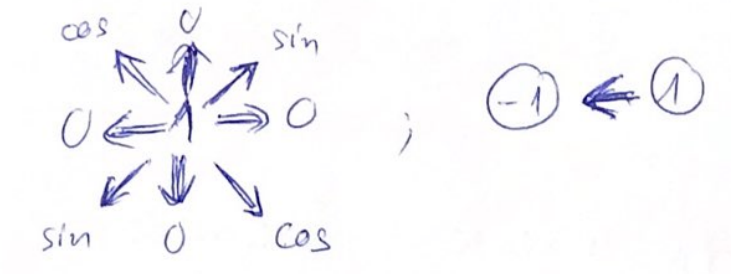
\includegraphics[width=0.5\textwidth]{elementary-rotation-matrix.png}
\end{figure}

\section{Position \& Orientation}
\begin{itemize}
	\item Euler angles: \textbf{12} different sets of angles $R_{xy'z''}(\Phi) = R_z(\varphi) R_{y'}(\theta) R_{z''}(\psi)$
	\item Roll-Pitch-Yaw: fixed frame $XYZ$ $R(\varphi, \theta, \psi) = R_z(\varphi) R_y(\theta) R_x(\psi)$
	\item Gimbal lock: loss of 1 \ac{dof} in a 3-dimensional, 3 gimbal mechanism when 2/3 gimbals are driven into a parallel configuration\\
	\note It exists no matter what rotation sequence you choose
	\item Angle \& axix representation: solves gimbal lock problem\\
	However, does not guarantee an unique solution. When doing inverse, has problem when $\sin \theta=0$
	\item Unit quaternion: \hlb{CAN} describe any rotation without ambiguities!
\end{itemize}
\hlb{Intuition:} angle \& axis representation, unit quaternion are ways to avoid dealing with/or deal better with gimbal lock

\section{Actuators and Joints}
\section{Workspace}

\section{Kinematics}
\subsection{Direct Kinematics}
\begin{itemize}
	\item Homogeneous coordinate representation, transformation matrix
	\item $\vec{e}_{x, \prescript{i}{}{o}} = \vec{e}_{z, \prescript{i-1}{}{o}} \times \vec{e}_{z, \prescript{i}{}{o}}$
\end{itemize}

\subsection{Inverse Kinematics}
\begin{itemize}
	\item Kinematic redundancy: No $\rightarrow$ Functional $\rightarrow$ hyper
	\item 3 ways to solve:
	\begin{itemize}
		\item Analytical: if analytical solution exists, \hlb{ALWAYS} use it. Non redundant
		\item Numerical: If closed-form solution does not exist / too hard to find analytically. If redundant
		\begin{align*}
			err &= r_d - f(q_e)\\
			q_{k+1} &= q_k + \frac{1}{J_A(q)} adj(J_A(q)) err_k
		\end{align*}
		\item Algebraic: solve polynomials equations
	\end{itemize}
\end{itemize}

\subsection{Differential Kinematics}
{\color{red} \boxed{\text{joint velocity $\Rightarrow$ \ac{ee} velocity}}}

\hlb{Using Geometric Jacobian}
\begin{align}
	&q = [q_1 \dots q_n]^T &&-\text{joint positions}\\
	&v_E = \begin{bmatrix}
		\dot{p}_E\\
		\omega_E
	\end{bmatrix} &&-\text{\ac{ee} velocity}\\
	&\dot{p}_E = [\dot{p}_x \quad \dot{p}_y \quad \dot{p}_z]^T &&-\text{\ac{ee} linear velocity}\\
	&\omega_E = [\omega_x \quad \omega_y \quad \omega_z]^T &&-\text{\ac{ee} angular velocity}\\
	\Rightarrow & v_E = J_G(q).\dot{q}\\
	&J_G(q) = \begin{bmatrix}
		J_{GP}(q)\\
		J_{GO}(q)
	\end{bmatrix} && \begin{matrix*}[l]
	-\text{Geometric Jacobian}\\
	J_{GP}(q) - \text{geometric position Jacobian}\\
	J_{GO}(q) - \text{geometric orientation Jacobian}
\end{matrix*}
\end{align}

\hlb{Using Velocity Composition Rule}
\begin{itemize}
	\item Linear velocity composition rule
	\begin{align}
		\prescript{O}{}{\dot{r}_{p, \prescript{0}{}{O}}} = 
	\end{align}
	\item Angular velocity composition rule
	\item Strictly follow \ac{DH} conventions, then $\Rightarrow \delta, d, l, \alpha, \theta$\\
	Prismatic joints, revolute joints
\end{itemize}

\subsection{Kinematics Singularities}
Kinematics singularities occurs if the Jacobian is rank-deficient. There are 2 types:
\begin{itemize}
	\item Boundary singularities: manipulator is out stretched or retracted $\Rightarrow$ does not drive the robot to the edge
	\item Internal singularities: caused by alignment of 2/more axes
\end{itemize}

Singularity affects the kinematics solution:
\begin{itemize}
	\item Mobility of robotic structure is reduced
	\item Inverse kinematics $\Rightarrow$ yields infinite solutions
	\item Close to a singularity, small velocity in operational space \hlr{CAUSES} large velocity in joint space
\end{itemize}

\todo{Singularities decoupling \hlr{$\star$}}

\subsection{Kinematic Redundancy}
\subsection{Differential Mapping}
\subsection{Inverse Differential Kinematics}
\subsection{Statics}

\subsection{Manipulability Ellipsoids}

\section{Dynamics Model}
\section{Dynamic Parameter Identification}
\section{Direct \& Inverse Dynamics}
\section{Parallel Kinematics}
	% !TeX spellcheck = en_US
\chapter{Trajectory Planning}

\section{Introduction}

\subsection{Definitions}
\hlr{Goal:} compute a function of time that describes the motion of robot's joints. Depending on the task and time constraints, there will be different restrictions on the trajectory.
\begin{itemize}
	\item A {\color{blue} \textbf{Path}} is a set of points in the joint/operational space, as geometrical description of the motion
	\item A {\color{red} \textbf{Trajectory}} is a path through space as a function of time\\
	\textbf{{\color{red} \boxed{\text{Trajectory = Path + Time Law}}}}
\end{itemize}

\subsection{Joint space vs. Operational Space Trajectory Planning}
\begin{itemize}
	\item Joint space: planning is done in terms of joint positions, velocities and accelerations: ${\color{red} q, \dot{q}, \ddot{q}}$. $\Rightarrow$ trajectory of the \ac{ee} should NOT be important.
	\item Operational space: planning is done in terms of \ac{ee} positions, orientation and their derivatives: ${\color{blue} \textbf{x}_E, \dot{\textbf{x}}_E, \ddot{\textbf{x}}_E}$. This gives more control over the \ac{ee} path, \eg, for melding, gluing applications.
\end{itemize}

\begin{figure}[hbt!]
	\centering
	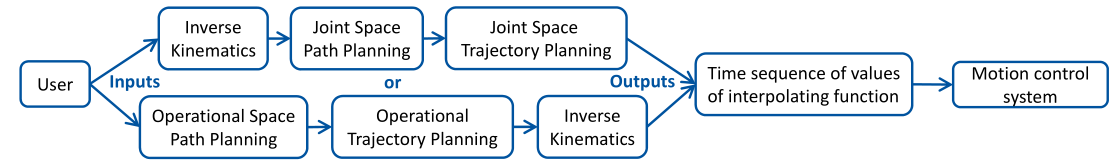
\includegraphics[width=\textwidth]{trajectory-planning.png}
	\caption{Trajectory planning procedure.}
	\label{fig:trajectory-planning}
\end{figure}
\begin{itemize}
	\item Inputs: path description, geometric / kinematic constraints (usually in operational space), constraints resulting from the manipulator dynamics
	\item Outputs: A time sequence of values for the joints' positions, velocities and accelerations as needed by the motion control system
	\item The paths and trajectories are not defined by the user explicitly in each point, but as a set of relevant \ac{param}: start, end points, possible intermediate points, geometric primitives, total time, maximum accelerations and velocities
\end{itemize}

\section{Joint Space Trajectories}
Given start and end \ac{ee} poses $\textbf{P}_{start}, \textbf{P}_{end}$ (and possible intermediate poses), apply inverse kinematics to get the joint poses (\figref{fig:trajectory-planning}).
\begin{equation*}
	\left. \begin{matrix*}[l]
		{\color{blue} \textbf{P}_{start}} \Rightarrow {\color{red} \textbf{q}(t_{start})}\\
		{\color{blue} \textbf{P}_{end}} \Rightarrow {\color{red} \textbf{q}(t_{end})}
	\end{matrix*} \right\} \Rightarrow {\color{red} \textbf{q}_t, \dot{\textbf{q}}_t, \ddot{\textbf{q}}_t} \quad\text{for}\quad t\in[t_{start}, t_{end}]
\end{equation*}

\subsection{Point-to-Point Motion}
Possible \hlb{timing laws} for point-to-point motion:
\begin{itemize}
	\item Cubic polynomial for the joints motion: can impose start, end positions and velocities
	\begin{align*}
		&q_i(t) = a_{i,3}t^3 + a_{i,2}t^2 + a_{i,1}t + a_{i,0} &&-\text{cubic polynomial for joint $i$ motion}\\
		&\dot{q}_i(t) = 3a_{i,3}t^2 + 2a_{i,2}t + a_{i,1} &&-\text{parabolic velocity profile}\\
		&\ddot{q}_i(t) = 6a_{i,3}t + 2a_{i,2} &&-\text{linear acceleration profile}
	\end{align*}
	\hlb{Problem:} infinite jerk at start and end positions
	\begin{figure}[hbt!]
		\centering
		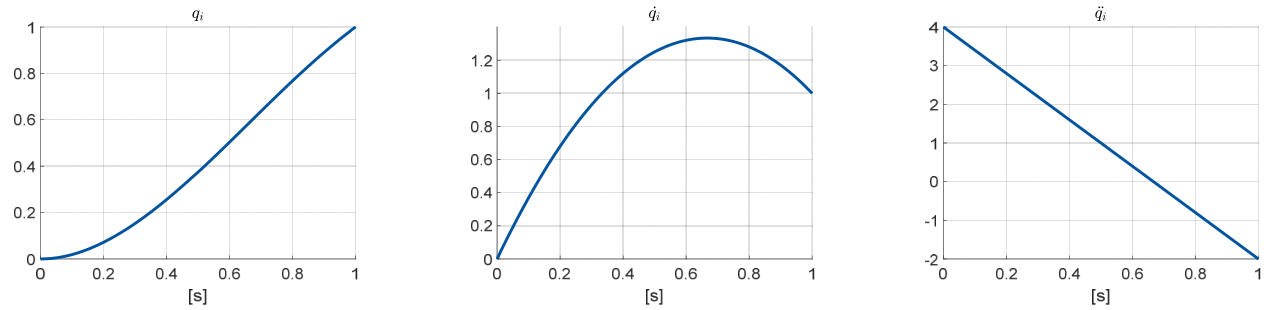
\includegraphics[width=\textwidth]{cubic-polynomial.png}
		\caption{Example of cubic polynomial.}
	\end{figure}
	\item Fifth order polynomial for the joints motion: allows imposing start, end positions, velocities and accelerations with finite jerk.
	\begin{align*}
		&q_i(t) = a_{i,5}t^5 + a_{i,4}t^4 + a_{i,3}t^3 + a_{i,2}t^2 + a_{i,1}t + a_{i,0} &&-\text{fifth order polynomial}\\
		&\dot{q}_i(t) = 5a_{i,5}t^4 + 4a_{i,4}t^3 + 3a_{i,3}t^2 + 2a_{i,2}t + a_{i,1} &&-\text{forth order velocity profile}\\
		&\ddot{q}_i(t) = 20a_{i,5}t^3 + 12a_{i,4}t^2 + 6a_{i,3}t + 2a_{i,2} &&-\text{cubic acceleration profile}
	\end{align*}
	\begin{figure}[hbt!]
		\centering
		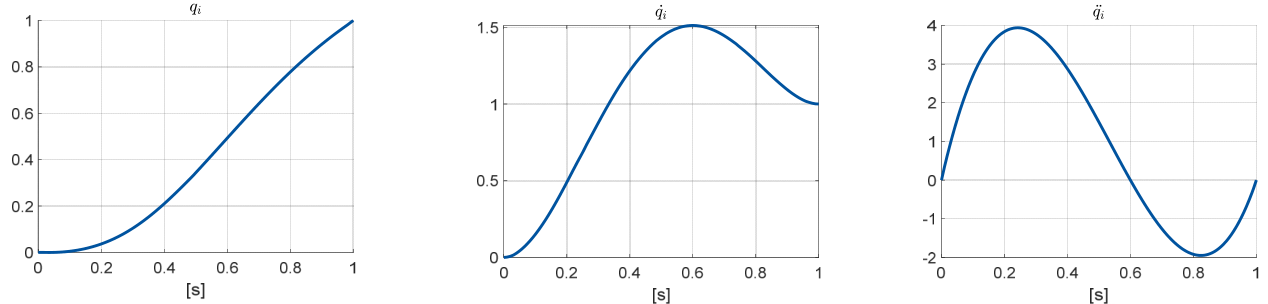
\includegraphics[width=\textwidth]{fifth-order-polynomial.png}
		\caption{Example of fifth order polynomial.}
	\end{figure}
	\item Trapezoidal acceleration profile: given time period, $\max$ acceleration, velocity and position.
	\note Just know that the below formulas and constraints exist. The derivation is complicated and time-consuming.
	\begin{align*}
		\Delta t_{i,I} &= T - \frac{\dot{q}_{\max}}{\ddot{q}_{\max}} - \frac{q_{\max}}{\dot{q}_{\max}} && \frac{q_{\max}}{T} \leq \dot{q}_{\max} \leq \frac{2q_{\max}}{T}\\
		\Delta t_{i,II} &= 2\frac{\dot{q}_{\max}}{\ddot{q}_{\max}} + \frac{q_{\max}}{\dot{q}_{\max}} -T && \frac{\dot{q}_{\max}}{T - \frac{q_{\max}}{\dot{q}_{\max}}} \leq \ddot{q}_{\max} \leq \frac{2\dot{q}_{\max}}{T - \frac{q_{\max}}{\dot{q}_{\max}}}\\
		\Delta t_{i,IV} &= T - 4 \Delta t_{i,I} - 2 \Delta t_{i,II} && \dddot{q}_{\max} = \frac{\ddot{q}_{\max}}{\Delta t_{i,I}} = \frac{\ddot{q}_{\max}}{T - \frac{\dot{q}_{\max}}{\ddot{q}_{\max}} - \frac{q_{\max}}{\dot{q}_{\max}}}\\
	\end{align*}
	\begin{figure}[hbt!]
		\centering
		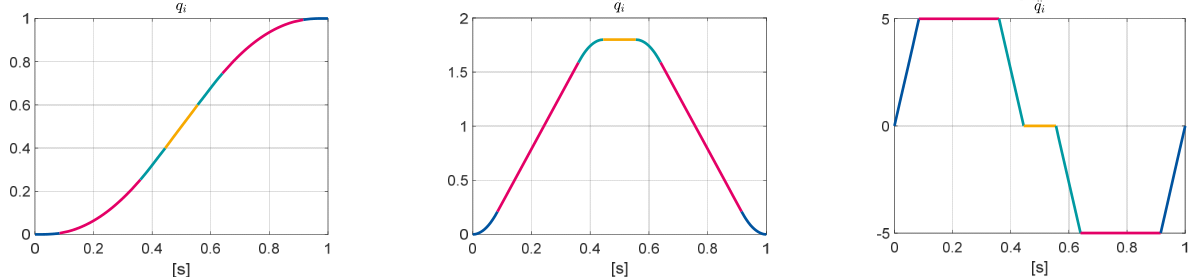
\includegraphics[width=\textwidth]{trapezoidal-acceleration-profile.png}
		\caption{Example of trapezoidal acceleration profile.}
	\end{figure}
\end{itemize}

\subsection{Motion through a Sequence of Points}
\begin{itemize}
	\item This can be viewed as extension of point-to-point motion
	\item The path is defined through a \textbf{sequence of $N$ path points}
	\item The time instances when these points must be reached should also be given
	\item Instead of using an $(N+3)$-order polynomial through $N$ joint configurations, we can use low-order interpolating polynomials (\figref{fig:interpolating-polynomials}).
	\begin{itemize}
		\item Each joint variable $q_i$ corresponds to a set of $N-1$ cubic polynomials $\Pi_{i,k}(t), k=1, \dots, N-1$
	\end{itemize}
	\begin{align*}
		q_i(t_k) &= q_{i,k} &&-\text{intermediate poses}\\
		q_{i,1} &= q_{i,start}, q_{i,N} = q_{i,end}\\
		t_{i,1} &= t_{i,start}, t_{i,N} = t_{i,end}\\
		\Pi_{i,k}(t_k) &= \Pi_{i,k+1}(t_k) = q_{i,k} &&-\text{path continuity}
	\end{align*}
	\item To impose \textbf{velocity continuity}, additional information is needed
	\[ \dot{\Pi}_{i,k}(t_{i,k+1}) = \dot{\Pi}_{i,k+1}(t_{i,k+1}) = \dot{q}_i(t_{i,k+1}) \]
	\begin{itemize}
		\item Arbitrary values for the velocity at the path points $\dot{q}_i(t_k)$ \textbf{or}
		\item Values for the velocity at the path points $\dot{q}_i(t_k)$ according to some criteria \textbf{or}
		\item Impose continuous acceleration at the path points
	\end{itemize}
	\note Probably leads to acceleration jerks
	\item Continuity for acceleration: imposed by 4 equations\\
	\note Required using 2 additional virtual points for 2 additional polynomials $\Rightarrow 4(N+1)$ equations for $4(N+1)$ unknowns. It is computationally expensive. With some tricks, the problem can be reduced to $N$ variables \dots
\end{itemize}

\begin{figure}[hbt!]
	\centering
	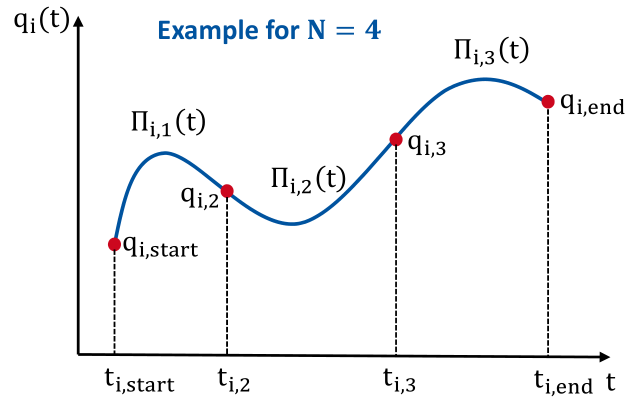
\includegraphics[width=0.5\textwidth]{interpolating-polynomials.png}
	\caption{Example of motion through sequence of four points using low-order (cubic) interpolating polynomials.}
	\label{fig:interpolating-polynomials}
\end{figure}

\section{Operational-space Trajectories}
\begin{itemize}
	\item Planning in the Joint Space may result in unexpected \ac{ee} motion, resulting from the non‐linear direct kinematics.
	\item Planning in Operational Space ensures that the \ac{ee} motion follows exactly the geometrically specified path by
	\begin{itemize}
		\item interpolating a sequence of prescribed poses
		\item generating analytical motion primitives (e.g. lines, circular arcs etc.)
		\item but it requires \hlr{real time} inverse kinematic computation, which is more computationally expensive
	\end{itemize}
	\item {\color{red}\boxed{\text{Path primitives + timing laws = trajectory planning}}}\\
	analyzed and computed separately
\end{itemize}

\subsection{Path primitive}
\begin{itemize}
	\item The word \textit{primitive} means a basic component, from which other is derived.
	\item \hlr{Path primitives} are the analytical geometrical descriptions for paths.
	\item Parametric representation of the path $\Gamma$ in space is a function of a general parameter $\sigma$ describe the position vector for point $\textbf{P}$ (\figref{fig:path-parametric-representation})
	\[ \textbf{r}_{\textbf{P}, \prescript{j}{}{O}} = \textbf{r}_\textbf{P} = \textbf{r}_\textbf{P}(\sigma), \quad \sigma\in[\sigma_{start}, \sigma_{end}]\]
	\item Usually it makes sense to replace general \ac{param} $\sigma$ by the current path length $s$
	\[ \textbf{r}_\textbf{P}(s) = f(s) \quad\text{with}\quad \sigma_{start}=0, \sigma_{end} = s_{end} \]
\end{itemize}

\begin{figure}[hbt!]
	\centering
	\begin{minipage}{0.45\textwidth}
		\centering
		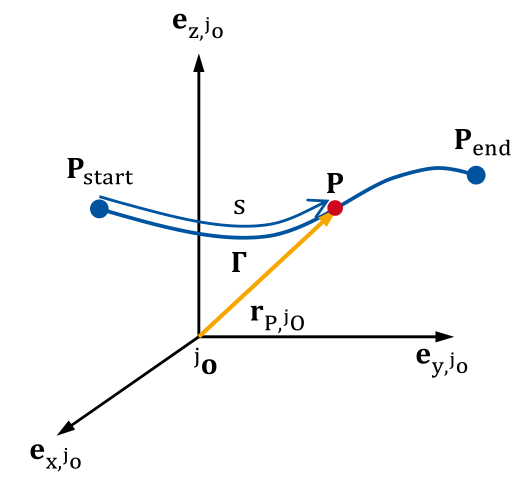
\includegraphics[width=\textwidth]{path-parametric-representation.png}
		\caption{Example for parametric representation of path $\Gamma$}
		\label{fig:path-parametric-representation}
	\end{minipage}\hfill
	\begin{minipage}{0.45\textwidth}
		\centering
		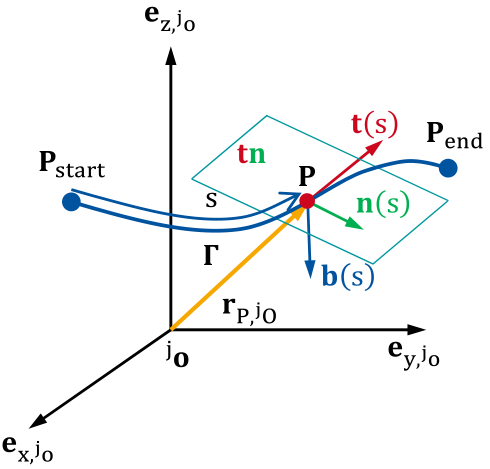
\includegraphics[width=\textwidth]{frenet-frame.png}
		\caption{Frenet frame with 3 unit vectors.}
		\label{fig:frenet-frame}
	\end{minipage}
\end{figure}

\subsection{Frenet Frame}
Frenet Frame is used to define the coordinate orientation along the path $\Gamma$. The three unit vectors establish the Frenet frame (\figref{fig:frenet-frame}):
\begin{itemize}
	\item Tangent unit vector $\displaystyle {\color{red} \textbf{t}(s)} = \frac{d\textbf{r}_P(s)}{ds} $ along the direction of the path
	\item Normal unit vector $\displaystyle {\color{Green} \textbf{n}(s)} = \frac{1}{\left|\left| \frac{d^2 \textbf{r}_P(s)}{ds^2} \right| \right|} \frac{d^2 \textbf{r}_P(s)}{ds^2} $ perpendicular to ${\color{red} \textbf{t}(s)}$
	\item Binormal unit vector $\displaystyle {\color{blue} \textbf{b}(s)} = {\color{red} \textbf{t}(s)} \times {\color{Green} \textbf{n}(s)}$ complements a right handed moving frame
\end{itemize}

\subsection{Path Primitive: Rectilinear Path}
The simplest parametric path representation is a linear segment between $\textbf{P}_{start}$ and $\textbf{P}_{end}$
\begin{align}
	\textbf{r}_{P,\prescript{j}{}{O}}(s) &= \textbf{r}_{P_{start}, \prescript{j}{}{O}} + \frac{s}{\left|\left| \textbf{r}_{P_{end}, \prescript{j}{}{O}} - \textbf{r}_{P_{start}, \prescript{j}{}{O}} \right|\right|} \left( \textbf{r}_{P_{end}, \prescript{j}{}{O}} - \textbf{r}_{P_{start}, \prescript{j}{}{O}} \right)\\
	{\color{red} \textbf{t}(s)} &= \frac{d\textbf{r}_P(s)}{ds} = \frac{1}{\left|\left| \textbf{r}_{P_{end}, \prescript{j}{}{O}} - \textbf{r}_{P_{start}, \prescript{j}{}{O}} \right|\right|} \left( \textbf{r}_{P_{end}, \prescript{j}{}{O}} - \textbf{r}_{P_{start}, \prescript{j}{}{O}} \right)\\
	{\color{Green} \textbf{n}(s)} &= \frac{1}{\left|\left| \frac{d^2 \textbf{r}_P(s)}{ds^2} \right| \right|} \frac{d^2 \textbf{r}_P(s)}{ds^2} \quad\text{with}\quad \frac{d^2 \textbf{r}_{P,\prescript{j}{}{O}}(s)}{ds^2}=0
\end{align}
$\Rightarrow$ \hlr{CAN NOT} define the Frenet frame uniquely. The plane ${\color{red}\textbf{t}\color{Green}\textbf{n}}$ can be rotated arbitrarily around ${\color{red} \textbf{t}(s)}$

\begin{figure}[hbt!]
	\centering
	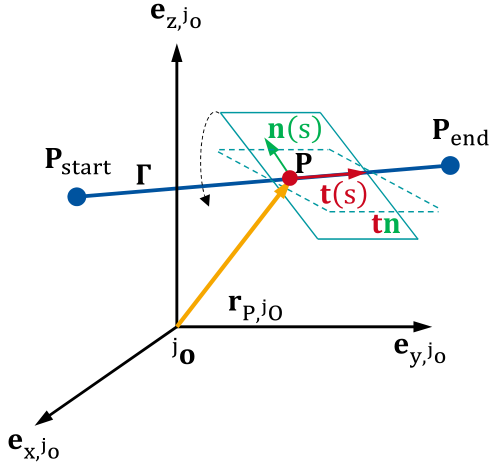
\includegraphics[width=0.3\textwidth]{rectilinear-path.png}
	\caption{Rectilinear path primitive.}
	\label{fig:rectilinear-path}
\end{figure}

\subsection{Path Primitive: Circular Arc}
The circular arc is defined through three points $\textbf{P}_{start}$, $\textbf{P}_{mid}$ and $\textbf{P}_{end}$.

\begin{minipage}{.5\textwidth}
	\begin{itemize}
		\item Compute center $\prescript{j}{}{\textbf{r}}_{\prescript{C}{}{O}, \prescript{j}{}{O}}$
		\begin{itemize}
			\item Determine $\prescript{j}{}{\textbf{r}}_{P_{mid}, P_{start}}$
			\item Determine $\prescript{j}{}{\textbf{r}}_{P_{end}, P_{start}}$
			\item Determine unit vector $\prescript{j}{}{\textbf{e}}_{z,\prescript{C}{}{O}}$
			\item Determine helper vectors $\textbf{r}_{H_1}, \textbf{r}_{H_2}$
			\item Determine $\prescript{j}{}{\textbf{r}}_{\prescript{C}{}{O}, \prescript{j}{}{O}}$
		\end{itemize}
		\item Determine unit vectors $\prescript{j}{}{\textbf{e}}_{x,\prescript{C}{}{O}}, \prescript{j}{}{\textbf{e}}_{y,\prescript{C}{}{O}}$
		\item Determine radius
		\item \dots
	\end{itemize}
\end{minipage}
\begin{minipage}{.45\textwidth}
	\centering
	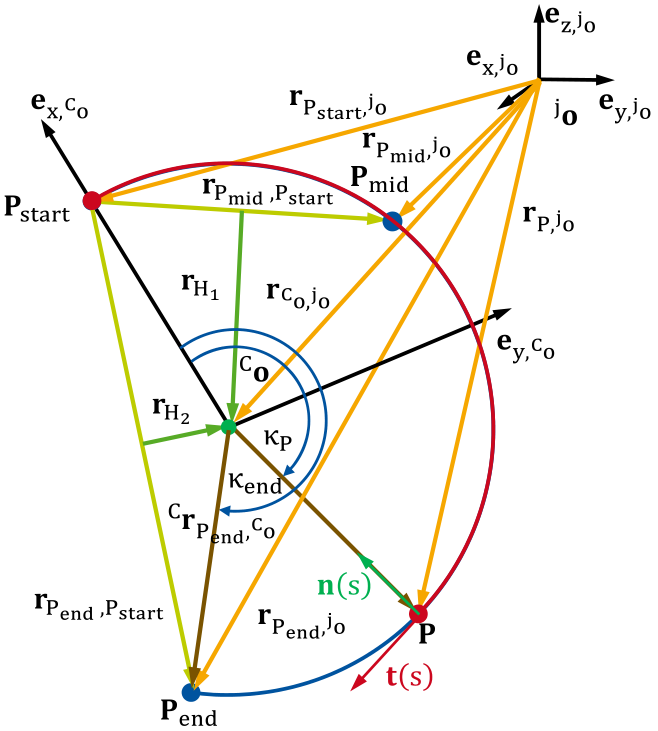
\includegraphics[width=\textwidth]{circular-arc.png}
\end{minipage}

\subsection{Path Primitive: Spline Path}
Given a set of points $\textbf{P}_i$ for $i\in\{1,n\}$, a smooth curves is generated by interpolating method
\begin{itemize}
	\item Between two consecutive points $\textbf{P}_i$ and $\textbf{P}_{i+1}$, there is path segment $\textbf{S}_i(\lambda)$
	\item To ensure smoothness between path's segments, the path must be continuous up to its second derivative at path points
	\item Use polynomials of degree five
	\[\textbf{S}_i(\lambda) = a_{i,5} \lambda^5 + a_{i,4} \lambda^4 + a_{i,3} \lambda^3 + a_{i,2} \lambda^2 + a_{i,1} \lambda + a_{i,0}, \qquad 0\leq \lambda \leq \lambda_i \]
\end{itemize}

\begin{figure}[hbt!]
	\centering
	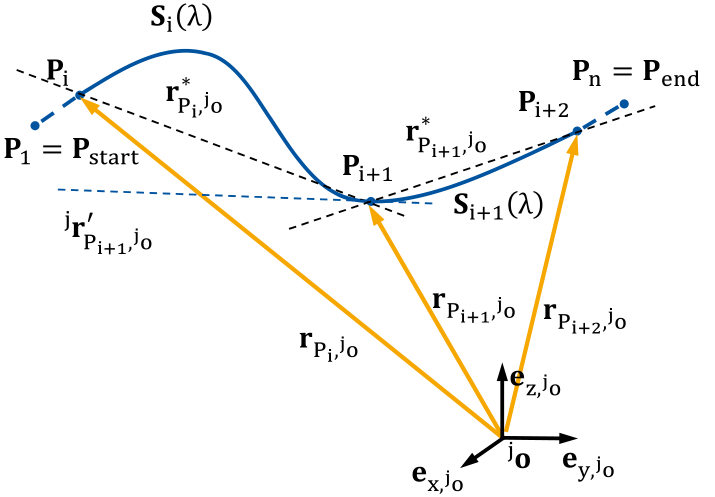
\includegraphics[width=0.5\textwidth]{spline-path.png}
	\caption{Spline path primitive.}
	\label{fig:spline-path}
\end{figure}

\section{Nonlinear Dynamics Motor Primitives}
This \textit{nonlinear dynamics motor primitives} are NOT the same as path primitives mentioned above. Let's examine two second-order dynamic systems $(z,y)$ and $(v,x)$ as follows: \cite{ijspeert2002movement}
\begin{align}
	\dot{z} &= f_z(y,z) = \alpha_z (\beta_z (g-y) - z)\\
	\dot{y} &= f_y(z,x,v) = z + \frac{\sum_{i=1}^N \Psi_i w_i}{\sum_{i=1}^N \Psi_i} v\\
	\dot{v} &= f_v(x,v) = \alpha_v (\beta_v (g-x) -v)\\
	\dot{x} &= f_x(v) = v\\
	\Psi_i &= \exp \left( -\frac{1}{2\sigma_i^2} (\tilde{x}-c_i)^2 \right), \quad i = 1, \dots, N &&-\text{Gaussian kernel functions}\\
	\tilde{x} &= \frac{x - x_0}{g - x_0}
\end{align}
\begin{itemize}
	\item The 2nd system dynamic behavior is simply analogous to value tracking: variable $x$ goes to target value $g$, the velocity $v$ starts and ends at 0 (\figref{fig:trajectory-tracking-1}).
	\item Compared to the 2nd one, the 1st system is just different in the extra nonlinear term in $\dot{y}$
	\item This is similar as with Fourier series. Fourier series is used to approximate an arbitrary time series data via a weighted sum of multiple sinusoidal functions. Here, we approximate the different between the velocity profile for trajectory tracking and for value tracking by a weighted sum of Gaussian-like functions.
	\item The above dynamical system is spatially invariant in the sense that scaling of the goal $g$ does not affect the topology of the attractor landscape
\end{itemize}

\begin{figure}[hbt!]
	\centering
	\begin{minipage}{0.49\textwidth}
		\centering
		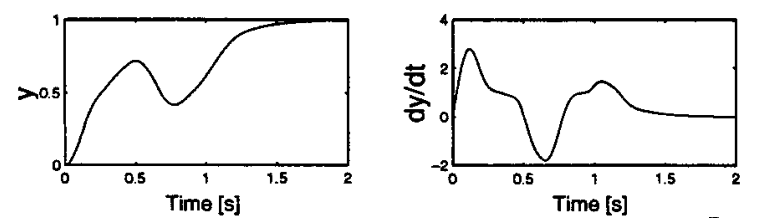
\includegraphics[width=\textwidth]{trajectory-tracking.png}
		\caption{Trajectory tracking: $y$ as joint position and velocity profile $\dot{y}$.}
		\label{fig:trajectory-tracking}
	\end{minipage}\hfill
	\begin{minipage}{0.49\textwidth}
		\centering
		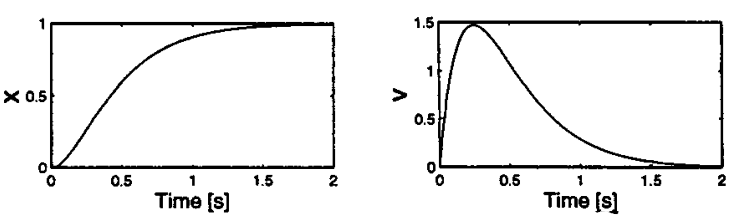
\includegraphics[width=\textwidth]{trajectory-tracking-1.png}
		\caption{Value tracking: $x$ as joint position and velocity profile $\dot{x}$.}
		\label{fig:trajectory-tracking-1}
	\end{minipage}
	\begin{minipage}{0.4\textwidth}
		\centering
		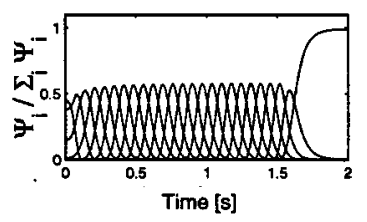
\includegraphics[width=\textwidth]{trajectory-tracking-2.png}
		\caption{Basis functions from Gaussian kernels.}
		\label{fig:trajectory-tracking-2}
	\end{minipage}
\end{figure}

With regards to trajectory planning, long story short, we manage to parameterize a trajectory $y$ to \ac{param} $w_i$
\begin{itemize}
	\item $q$ - current joint position
	\item $g$ - desired joint position
	\item $x$ - a timing signal
	\item $v$ - a scaling signal
\end{itemize}

Given a new trajectory:
\begin{itemize}
	\item Shift the given trajectory to $0$ start position
	\item Scale the time constants of the dynamical system such that $(v,x)$ reaches $(0,g)$ at approximately the same time $\Rightarrow$ a time trajectory for $v(t),x(t)$
	\item Given $v(t),x(t)$, calculate $u_{des} = \dot{y}_{demo} - z$ as desired output
	\item Learn $w_i$ via recursive least squares to minimize the locally weighted error criterion for each local model $u_{i,t} = w_i v_t$
	\[J_i = \sum_t \Psi_{i,t} (u_{des,t} - u_{i,t})^2\]
\end{itemize}

This parameterization approach satisfies following requirements: 
\begin{itemize}
	\item Able to fit a demonstrated trajectories with high precision (fitting all \ac{dof} and all points of the trajectories)
	\item Able to generate similar movements to different goals. If we fix the weights $w_i$, change the goal $g$, we will receive a similar trajectories. \note good with close targets, better with variation in height, not with left and right.
	\item Robust against perturbations (\eg, in scenarios there is interaction with external objects)
	\begin{align}
		&\tilde{y} &&-\text{the actual position}\\
		&\dot{y} = \alpha_y \left( \frac{\sum_{i=1}^N \Psi_i, w_i}{\sum_{i=1}^N \Psi_i} v + z \right) + \alpha_{py} (\tilde{y} - y)\\
		&\dot{x} = v \left( 1+ \alpha_{px}(\tilde{y}-y)^2 \right) ^{-1}
	\end{align}
	\item Good basis for comparing movements, as a metric for measuring differences between movements. Similar movements will have similar weights $w_i$ $\Rightarrow$ can be used to classify movements (simple nearest neighbors)
\end{itemize}

\todo{The effect of hyper-\ac{param}}
\begin{itemize}
	\item $\alpha_v$
	\item $\beta_v$
	\item $\alpha_z$
	\item $\beta_z$
	\item $c_i$
	\item \dots
\end{itemize}
	\include{Contents/advanced-robotics.tex}
	% !TeX spellcheck = en_US
\chapter{Robotics System Engineering}

\section{Structural Synthesis}

\section{End-Effector Technology}

\section{Components of Robotics System}

\section{Control Architecture}

\section{Mobile Manipulators}
	% !TeX spellcheck = en_US
\chapter{Robotics Sensor Systems}
This chapter gives an overview on different types of sensors used in robotic systems, the physics behind them and more \dots

\section{Overview}
Two classes of sensors:
\begin{table}[hbt!]
	\centering
	\begin{tabular}{p{8cm}|p{8cm}}
		Proprioceptive sensors & Exteroceptive sensors \\\hline\hline
		\textit{Proprioception}, also referred to as \textit{kinaesthesia}, is the sense of self-movement, force, and body position \href{https://en.wikipedia.org/wiki/Proprioception}{(src)}. & \textit{Exteroception} is sensitivity to stimuli that are outside the body, resulting from the response of specialized sensory cells to objects and occurrences in the external environment. Exteroception includes the five senses of sight, smell, hearing, touch, and taste \href{https://dictionary.apa.org/exteroception}{(src)}.\\ \hline
		\textit{Proprioceptive} sensors provide internal perception about the state of the robot, \ie, joint positions, velocities, accelerations, torque. & \textit{Exteroceptive} sensors provide external perception about the measured force, tactile input, proximity range, vision, \etc.
	\end{tabular}
\end{table}

\subsection{Future Applications}
\begin{itemize}
	\item Industrial robots: more complex tasks, wider / broader range of manufacturing
	\item Service robots: excluding industrial automation application
	\item Application: logistics, medical, field, defense robots.
\end{itemize}

\subsection{Key abilities} (CIMMPC)
\begin{itemize}
	\item Configurability
	\item Interaction ability
	\item Motion ability
	\item Manipulation ability
	\item Perception ability: suitable choice of sensing modality
	\item Cognitive ability: reduction of programming and configuration effort
\end{itemize}

\subsection{Key technologies}
Advances in sensors: $\begin{cases}
	- \text{Control theory}\\
	- \text{Safety}\\
	- \text{Navigation}
\end{cases}$

\todo{add graph}

\section{Control \& Feedback Control Systems}
\subsection{Introduction to industrial robots}
\subsection{Internal metrology of industrial robot}
\subsection{External metrology of industrial robot}
\subsection{Communication between sensors \& robots via industrial Ethernet \& 5G}

\section{Electromagnetic Sensor}
Proprioceptive sensors:
\begin{table}[hbt!]
	\centering
	\begin{tabular}{l|c|c|c}
		& Encoders & Tachometer & Gyroscope\\ \hline\hline
		Position/Pose & \checkmark &\\\hline
		Velocity & \checkmark & \checkmark\\\hline
		Acceleration & \checkmark & \checkmark & \checkmark
	\end{tabular}
\end{table}

\note If you can measure $x$, you can derive $\dot{x}, \ddot{x}$
\subsection{Principles of Electromagnetism}
\hlr{Maxwell's equations:}
\begin{itemize}
	\item Gauss's law
	\begin{align}
		\Phi_E = &\oint \vec{E}.d\vec{A} = \frac{Q_{encl}}{\varepsilon_0}; \varepsilon_0 = \text{const} &&\Leftrightarrow\quad \vec{\nabla}\vec{E} = \frac{\rho}{\varepsilon_0}\\
		\Leftrightarrow &\oint \vec{D}.d\vec{A} = \int \rho.dV = Q_{encl}; \vec{D} = \varepsilon \vec{E} &&\Leftrightarrow\quad {\color{red} \boxed{\color{black} \vec{\nabla} \vec{D} = \rho}}
	\end{align}
	\begin{align*}
		&\text{with:} &&\Phi_E - \text{electric flux}
	\end{align*}
	\item Gauss's law for magnetism: $\vec{B}$ is solenoidal vector fields. There is no magnetic monopole \todo{} \hlr{divergence, no source, no sink}
	\begin{align}
		&\Phi_B = \oint \vec{B}.d\vec{A} = 0 &&\Leftrightarrow\quad {\color{red} \boxed{\color{black} \vec{\nabla}\vec{B} = 0}}
	\end{align}
	\begin{align*}
		&\text{with:} &&\Phi_B - \text{magnetic flux}
	\end{align*}
	\item Maxwell-Faraday equation
	\item Ampere's circuital law
	\item Magnetic field
	\item Hall effect
\end{itemize}
\subsection{Position Sensors}
\begin{itemize}
	\item Potentiometer: works according to Ohm's law\\
	$\begin{cases}
		\text{Turning}\\
		\text{Sliding}
	\end{cases}$ potentiometer: when the joint rotates, the gear turns the potentiometer
	\item Induction-based sensors:
	\begin{itemize}
		\item Resolver \dots
		\item Inductive transducer
		\item Tranverse armature transducer: based on Maxwell's bridge
		\item Differential transducer
		\item Inductosyn
	\end{itemize}
	\item Rotary encoders:
	\begin{itemize}
		\item Absolutely Encoder \ac{vs} Incremental Encoder \todo{images}
		\begin{table}[hbt!]
			\centering
			\begin{tabular}{p{7cm}|p{7cm}}
				Absolutely Encoder & Incremental Encoder\\\hline\hline
				maintain \ac{info} when power is removed & immediately report position changes\\
				position \ac{info} is available immediately & doesn't keep track\\
				relationship between encoder value \& physical position set at assembly & have to go back to fixed point to initialize measurement
			\end{tabular}
		\end{table}
		\item Magnetic encoder \ac{vs} Optical encoder
		\item Number of track $\Rightarrow$ resolution\\
		$n$ tracks $\Rightarrow$ resolution $\frac{2\pi}{2_n}$
	\end{itemize}
\end{itemize}
\begin{table}[hbt!]
	\centering
	\begin{tabular}{c|c|c}
		& Advantages & Disadvantages\\ \hline\hline
		\multirow{2}{*}{Potentiometer} & Simple & Limited range \& accuracy\\
		& Low cost & Wear out (due to contact)\\ \hline
		\multirow{2}{*}{Resolver} & \multirow{2}{*}{Non-contact} & Analog, expensive\\
		& & Requires decoding circuit\\ \hline
		\multirow{2}{*}{Inductive Transducer} & Non-contact & limited range\\
		& High accuracy & Analog\\ \hline
		\multirow{2}{*}{Magnetic encoder} & Non-contact & Required decoding\\
		& Robust & usually lower resolution\\ \hline
		\multirow{2}{*}{Optical encoder} & \multirow{2}{*}{Non-contact} & Required gray decoding\\
		& & Complex wiring
	\end{tabular}
\end{table}

\note Current robots use encoders (magnetic / optical).

\subsection{Speed Sensors}
\hlr{Maxwell-Faraday's equation:}
\[\frac{\partial \vec{B}}{\partial t} \Rightarrow \frac{\partial \vec{E}}{\partial t}\]
\subsection{Acceleration Sensors}
\begin{itemize}
	\item Mechanical gyroscopes \hlr{(conservation of angular momentum)}
	\item Micro electro-mechanical system gyroscope (MEMS)
\end{itemize}

\section{Capacitive \& Piezoelectric Sensors}
\label{sec:capacitive-piezoelectric-sensors}

\section{Visual Electromagnetic Sensors}

\section{Thermoelectric \& Ultrasonic Sensors}

\section{Machine Vision}

\section{Tactile Information}

Types of robotic tactile sensors:
\begin{itemize}
	\item Capacitive tactile sensors (\secref{sec:capacitive-piezoelectric-sensors})
	\item Piezoresistive tactile sensors (\secref{sec:capacitive-piezoelectric-sensors})
	\item Piezoelectric tactile sensors (\secref{sec:capacitive-piezoelectric-sensors})
	\item Inductive tactile sensors
	\item Optical-based tactile sensors
	\begin{figure}[hbt!]
		\centering
		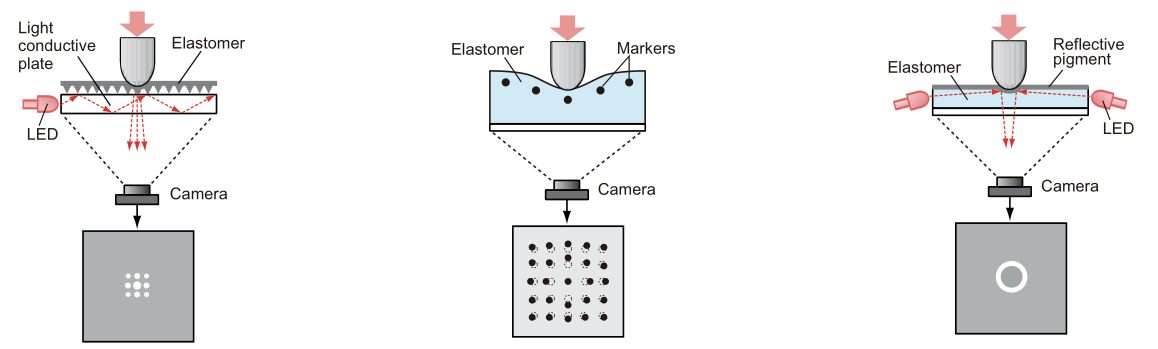
\includegraphics[width=\textwidth]{optical-tactile-sensors.png}
		\caption{Types of optical-based tactile sensors: Light conductive plate, Marker displacement, Reflective membrane (from left to right) \cite{shimonomura2019tactile}.}
	\end{figure}
	\item Strain gauges
	\item Audio-based tactile sensors: can provide information about surface texture.
	\item Multi-component tactile sensors
\end{itemize}
Prior works use tactile sensors in inference of object properties \cite{luo2017robotic} and robotic manipulation \cite{yamaguchi2019recent}.
\begin{itemize}
	\item Grasping
	\begin{itemize}
		\item Heuristic grasp adaptation strategy
		\item Grasp adaptation with slip detection
		\item Grasp adaptation with estimating friction coefficient
		\item Grasp adaptation with grasp stability estimation
		\item Complete grasp process with tactile sensing
	\end{itemize}
	\item Other robotic manipulation
	\begin{itemize}
		\item Detecting events with tactile sensors
		\item Estimating pose and location with tactile sensors
		\item Reinforcement learning with tactile sensors
		\item Exploring the workspace without vision
	\end{itemize}
	\item Tactile perception
\end{itemize}

Issues of introducing tactile sensors to robotic hands:
\begin{itemize}
	\item Difficulty to install on robotic hands.
	\item Wiring, power supply, and processing.
	\item Low durability, fragility.
	\item Less compatibility with the other tactile sensors.
	\item It is unclear what we can do with tactile sensors.
	\item Disadvantages caused by tactile sensors.
	\begin{itemize}
		\item Maintenance becomes complicated.
		\item Programming becomes complicated.
	\end{itemize}	
	\item Expensive.
	\item Asking for the moon.
\end{itemize}

\section{Data Acquisition \& Sensor Fusion}

\section{Signal Preprocessing}

\section{Communication \& Signal Transmission}
\subsection{Challenges in Data Transmission}
\begin{itemize}
	\item Different forms (text, speech, images)
	\item Large distances, limited time
	\item Certain bandwidth
\end{itemize}

\subsection{Information Systems \& Data Transmission Principles}
\subsection{Transmission Media}
\subsection{Network Topologies \& Data Transmission Protocols}
Topologies: $\begin{matrix*}[l]
	- \text{P2P}\\
	- \text{Bus}\\
	- \text{Fieldbus}
\end{matrix*}$

Protocols: OSI and TCP/IP

\subsection{Robot Communication with ROS}
	% !TeX spellcheck = en_US
\chapter{Probabilistic Robotics}

Reference from the great book: \cite{thrun2006probalistic}.

\section{State Estimation}
\subsection{Bayes Filters}
\begin{align*}
	&bel(x_t) = p(x_t | z_{1:t}, u_{1:t}) && \text{belief over a state}\\
	&\overline{bel}(x_t) = p(x_t | z_{1:t-1}, u_{1:t}) && \text{a posterior (before adapt to }z_t)\\
	\Rightarrow\; & \text{Calculating } bel(x_t) \text{ from  } \overline{bel}(x_t) && \text{correction/measurement update}
\end{align*}

\hlr{\underline{Bayes Filter Algorithm:}}
\begin{align*}
	&2 \qquad \text{for all } x_t \text{ do:}\\
	&3 \qquad \overline{bel}(x_t) = \int p(x_t | u_t, x_{t-1}) bel(x_{t-1}) dx && \text{prediction step}\\
	&4 \qquad bel(x_t) = \eta\, p(z_t | x_t)\, \overline{bel}(x_t) && \text{update step}
\end{align*}\\
$\Rightarrow\;$ Can only be implemented for very simple estimation problems, finite state space

\hlr{\underline{Important assumption:} Markov property} (each state s a complete summary of the past)

\hlr{Problem:} can not be implemented on digital computers

The next subsections describe two Gaussian filters (\ac{KF} and \ac{IF}) and two extensions of them (\ac{EKF} and \ac{EIF}). The Gaussian filters have major advantage in computational cost, with the disadvantage of having assumption on uni-model distribution.

\subsection{The Kalman Filter (KF)}

\begin{itemize}
	\item \hlb{Learning Resources:} \href{http://www.bzarg.com/p/how-a-kalman-filter-works-in-pictures/}{www.bzarg.com}
	\item For continuous space, not discrete or hybrid\\
	\item \hlr{Assumption:} posterior are Gaussians and Markov property\\
	\begin{align*}
		&p(x_t | u_t, x_{t-1}) && \text{must be linear \ac{func} (linear system dynamics)}\\
		&p(z_t, x_t) && \text{also linear}\\
		&bel(x_0) && \text{initial belief must be Gaussian}
	\end{align*}
\end{itemize}

\begin{align*}
	x_t &= A_t x_{t-1} + B_t u_t + \varepsilon_t\\
	p(x_t | u_t, x_{t-1}) &= \det \left( 2\pi\Sigma_t \right)^{-\frac{1}{2}} \exp\left[ -\frac{1}{2} \left( x_t - A_t x_{t-1} - B_t u_t \right)^T R_t^{-1} \left( x_t - A_t x_{t-1} - B_t u_t \right) \right]\\
	z_t &= C_t x_t + \delta_t \quad(=y)\\
	p(z_t | x_t) &= \det \left( 2\pi Q_t \right)^{-\frac{1}{2}} \exp\left[ -\frac{1}{2} \left( z_t - C_t x_t \right)^T Q_t^{-1} \left( z_t - C_t x_t \right) \right]\\
	bel(x_0) = p(x_0) &= \det \left( 2\pi\Sigma_0 \right)^{-\frac{1}{2}} \exp\left[ -\frac{1}{2} \left( x_t - \mu_0 \right)^T \Sigma_0^{-1} \left( x_t - \mu_0 \right) \right]
\end{align*}

\hlr{\underline{Kalman Filter Algorithm:}} $(\mu_{t-1}, \Sigma_{t-1}, u_t, z_t)$
\begin{align*}
	&\begin{rcases}
		2 \qquad \overline{\mu}_t = A_t \mu_{t-1} + B_t u_t\\
		3 \qquad \overline{\Sigma}_t = A_t \Sigma_{t-1} A_t^T + R_t \qquad\qquad\qquad\qquad\qquad\quad
	\end{rcases} \text{incorporate } u_t \text{ - prediction step - } \mathcal{O}(n^2)\\
	&\begin{rcases}
		4 \qquad K_t = \overline{\Sigma}_t C_t^T \left( C_t \overline{\Sigma}_t C_t^T + Q_t \right)^{-1} \qquad \text{(Kalman gain)}\\
		5 \qquad \mu_t = \overline{\mu}_t + K_t (z_t - C_t \overline{\mu}_t)\\
		6 \qquad \Sigma_t = (I - K_t C_t) \overline{\Sigma}_t
	\end{rcases} \text{incorporate } z_t \text{ - correction step - } \mathcal{O}(n^{2,8})\\
	&\;7 \qquad  \text{return } \mu_t, \Sigma_t \qquad\qquad\qquad\qquad\qquad\quad\qquad\qquad\Rightarrow\; \text{belief at time } t
\end{align*}
$\Rightarrow$ quite computationally expensive, \hlr{everything are Gaussians}

\subsection{Extended Kalman Filter (EKF)}
Overcome the assumption on linearity by only approximate by Gaussians
\begin{align*}
	x_t &= g(u_t, x_{t-1}) + \varepsilon_t\\
	z_t &= h(x_t) + \delta_t
\end{align*}

\begin{align*}
	g(u_t, x_{t-1}) &\approx g(u_t, \mu_{t-1}) + g'(u_t, \mu_{t-1}) (x_t - \mu_{t-1}) \\
	&= g(u_t, \mu_{t-1}) + G_t(x_t - \mu_{t-1})\\
	& g' \text{ is the Jacobian of state } (n\times n \text{ matrix})\\
	p(x_t | u_t, x_{t-1}) &\approx \det \left( 2\pi R_t \right)^{-\frac{1}{2}} \exp \left\{-\frac{1}{2} [x_t - g(u_t, x_{t-1})] ^T R_t^{-1} [x_t - g(u_t, x_{t-1})] \right\} \\
	h(t) &\approx h(\overline{\mu}_t) + h'(\mu_t) (x_t - \mu_{t-1})\\
	&= h(\overline{\mu}_t) + H_t (x_t - \mu_{t-1})\\
	p(z_t | x_t) &= \det \left( 2\pi Q_t \right)^{-\frac{1}{2}} \exp \left\{-\frac{1}{2} [z_t - h(x_t)] ^T Q_t^{-1} [z_t - h(x_t)]\right\} \\
\end{align*}

\hlr{\underline{Extended Kalman Filter Algorithm:}} $(\mu_{t-1}, \Sigma_{t-1}, u_t, z_t)$
\begin{align*}
	&2 \qquad \overline{\mu}_t = g(u_t, \mu_{t-1})\\
	&3 \qquad \overline{\Sigma}_t = G_t \Sigma_{t-1} G_t^T + R_t\\
	&4 \qquad K_t = \overline{\Sigma}_t H_t^T \left( H_t \overline{\Sigma}_t H_t^T + Q_t \right)^{-1} \\
	&5 \qquad \mu_t = \overline{\mu}_t + K_t [z_t - h(\overline{\mu}_t)]\\
	&6 \qquad \Sigma_t = (I - K_t H_t) \overline{\Sigma}_t\\
	&7 \qquad \text{return } \mu_t, \Sigma_t
\end{align*}

\begin{itemize}
	\item Can extend \ac{EKF} $\Rightarrow$ \ac{MHEKF}
	\item \ac{EKF}'s performance depends on degree of nonlinearities and uncertainty
	\item Unscented \ac{KF} and moments matching \ac{KF} are better
\end{itemize}

\subsection{Information Filter (IF)}
\begin{itemize}
	\item Moment representation:\tab\tab $\mu \quad\&\quad \Sigma$
	\item Canonical representation:\tab\tab $\xi \quad\&\quad \Omega$\\
	Information \ precision matrix: \tab $\Omega = \Sigma^{-1};\qquad \Sigma = \Omega^{-1}$\\
	Information vector: \tab \tab \tab $\xi = \Sigma^{-1}\mu;\qquad \mu = \Omega^{-1}\xi$
\end{itemize}
\begin{align*}
	p(x) &= \det(2\pi\Sigma)^{-\frac{1}{2}} \exp \left\{-\frac{1}{2} (x-\mu)^T \Sigma^{-1} (x-\mu) \right\}\\
	&= \eta \exp\left\{ -\frac{1}{2} x^T\Omega x + x^T \xi \right\}
\end{align*}

\hlr{\underline{Information Filter Algorithm:}} $(\xi_{t-1}, \Omega_{t-1}, u_t, z_t)$
\begin{align*}
	&\begin{rcases}
		2 \qquad \overline{\Omega}_t = (A_t \Omega_{t-1}^{-1} A_t^T + R_t)^{-1} \qquad\qquad\\
		3 \qquad \overline{\xi}_t = \overline{\Omega}_t ( A_t \Omega_{t-1}^{-1} \xi_{t-1} + B_t u_t )
	\end{rcases} \mathcal{O}(n^{2,8})\\
	&\begin{rcases}
		4 \qquad \Omega_t = C_t^T Q_t^{-1} C_t + \overline{\Omega}_t\\
		5 \qquad \xi_t = C_t^T Q_t^{-1} z_t + \overline{\xi}_t \qquad\qquad\qquad\quad
	\end{rcases} \mathcal{O}(n^2)\\
	&\;6 \qquad \text{return } \xi_t, \Omega_t
\end{align*}

\subsection{Extended Information Filter (IF)}
\begin{align*}
	x_t &= g(u_t, x_{t-1}) + \varepsilon_t\\
	z_t &= h(x_t) + \delta_t\\
	G_t &= g'(u_t, \mu_{t-1})\\
	H_t &= h'(\mu_t)
\end{align*}

\hlr{\underline{Extended Information Filter Algorithm:}} $(\xi_{t-1}, \Omega_{t-1}, u_t, z_t)$
\begin{align*}
	&2 \qquad \mu_{t-1} = \Omega_{t-1}^{-1} \xi_{t-1}\\
	&3 \qquad \overline{\Omega}_t = (G_t \Omega_{t-1}^{-1} G_t^T + R_t)^{-1}\\
	&4 \qquad \overline{\xi}_t = \overline{\Omega}_t\, g(u_t, \mu_{t-1})\\
	&5 \qquad \overline{\mu}_t = g(u_t, \mu_{t-1})\\
	&6 \qquad \Omega_t = \overline{\Omega}_t + H_t^T Q_t^{-1} H_t\\
	&7 \qquad \xi_t = \overline{\xi}_t + H_t^T Q_t^{-1} \left[ z_t - h(\overline{\mu}_t) - H_t \overline{\mu}_t \right]
\end{align*}

\begin{itemize}
	\item \hlb{Global uncertainty:} set $\Omega=0$ is better than set $|\Sigma| = \infty$
	\item \ac{IF} tends to be numerically more stable than \ac{KF}
	\item \ac{IF} is better for multi-robot problems
	\item For high dimensional state, \ac{EKF} is computational better than \ac{EIF}
\end{itemize}

\section{Measurements}
\subsection{Map Representation}
Maps: $m = \{ m_1, m_2, \dots, m_N \}$\\
\hlr{There are \underline{2 ways} to represent a map:}
\begin{table}[hbt!]
	\centering
	\begin{tabular}{c|c}
		feature-based & location-based \\\hline\hline
		$m_n$: properties of a feature and location of feature & a specific location \\\hline
		\hlr{only the shape} of the environment & volumetric: \hlr{label for any location} \\
		\hlr{at the specific locations} & in the world\\\hline
		easy to adjust positions of objects & occupancy grid map \\
		$\Rightarrow$ popular in the robotic mapping field &
	\end{tabular}
\end{table}

\todo{Add images}

\subsection{Measurement Noise}
The 4 types of measurement noise:
\begin{itemize}
	\item Correct range with local measurement noise\\
	With $z_t^{k*}$ as the correct distance
	\begin{equation}
		p_{hit}(z_t^k | x_t, m) = \begin{cases}
			\eta\; \mathcal{N}(z_t^k| z_t^{k*}, \sigma^2_{hit}) \qquad \text{if } 0 \leq z_t^k \leq z_{\max}\\
			0 \qquad\qquad\qquad\qquad\quad \text{otherwise}
		\end{cases}
	\end{equation}
	\item Unexpected object
	\begin{equation}
		p_{short}(z_t^k | x_t, m) = \begin{cases}
			\eta\lambda_{short} e^{-\lambda_{short} z_t^k} \qquad \text{if } 0 \leq z_t^k \leq z_t^{k*}\\
			0 \qquad\qquad\qquad\qquad \text{otherwise}
		\end{cases}
	\end{equation}
	\item Failures
	\begin{equation}
		p_{\max}(z_t^k | x_t, m) = I(z=z_{\max})
	\end{equation}
	\item Random measurements
	\begin{equation}
		p_{rand}(z_t^k | x_t, m) = \begin{cases}
			\frac{1}{z_{\max}} \qquad \text{if } 0 \leq z_t^k < z_{\max}\\
			0 \qquad\quad \text{otherwise}
		\end{cases}
	\end{equation}
\end{itemize}

\todo{Add image, plot}

\begin{equation}
	p(z_t^k | x_t, m) = \begin{bmatrix}
		z_{hit}\\ z_{short}\\
		z_{max}\\ z_{rand}
	\end{bmatrix}^T . \begin{bmatrix}
		p_{hit}(z_t^k | x_t, m)\\ p_{short}(z_t^k | x_t, m)\\
		p_{max}(z_t^k | x_t, m)\\ p_{rand}(z_t^k | x_t, m)
	\end{bmatrix}
\end{equation}

\section{Robot Motion}
Pose: $[x, y, \theta]^T$ at location $[x, y]^T$ and orientation $\theta$

\subsection{Motion Model}

Motion Model, \ac{aka} Probabilistic Kinematic Model: $p(x_t,  u_t, x_{t-1})$

\begin{table}[hbt!]
	\centering
	\begin{tabular}{c|c}
		Velocity commands & Odometry \\
		& (distance traveled, angle turned, \etc)\\\hline\hline
		& \hlr{more accurate}\\
		& \hlr{but post-the-fact}\\
		& \hlr{(not for motion planning)}\\
		Use for Probabilistic motion planning & Use for estimation
	\end{tabular}
\end{table}

Each has closed form calculation and sampling algorithm.

\subsection{Velocity Motion Model}
Assuming we can control a robot through velocities:
\begin{equation*}
	u_t = \begin{bmatrix}
		v_t\\ \omega_t
	\end{bmatrix}; \qquad
	x_{t-1} = \begin{bmatrix}
		x \\ y \\ \theta
	\end{bmatrix}; \qquad
	x_t = \begin{bmatrix}
		x'\\ y'\\ \theta'
	\end{bmatrix}
\end{equation*}

\hlr{\underline{Motion Model Velocity Algorithm:}} $(x_t, u_t, x_{t-1})$
\begin{align*}
	& \begin{rcases} \displaystyle
		2 \qquad \mu = \frac{1}{2} \frac{(x-x')\cos\theta+(y-y')\sin\theta}{(y-y')\cos\theta-(x-x')\sin\theta} \qquad\qquad\\
		3 \qquad x^* = \frac{x+x'}{2} + \mu (y-y')\\
		4 \qquad y^* = \frac{y+y'}{2} + \mu (x'-x)\\
		5 \qquad r^* = \sqrt{(x-x^*)^2 + (y-y^*)^2}
	\end{rcases} \text{Invert the motion model}\\
	& \;6 \qquad \Delta \theta = \text{atan2}(y'-y^*, x'-x^*) - \text{atan2}(y-y^*, x-x^*)\\
	& \begin{rcases}
		7 \qquad\hat{v} = \frac{\Delta\theta}{\Delta t} r^*\\
		8 \qquad\hat{\omega} = \frac{\Delta\theta}{\Delta t}\\
		9 \qquad\hat{\gamma} = \frac{\theta' - \theta}{\Delta t} - \hat{\omega}
		\qquad\qquad
	\end{rcases} \text{compared actual velocities with the desired}\\
	& 10 \qquad \text{return } p(v-\hat{v}, \alpha_1|v| + \alpha_2|\omega|) 
	\cdot p(\omega-\hat{\omega}, \alpha_3|v| + \alpha_4|\omega|)
	\cdot p(\hat{\gamma}, \alpha_5|v| + \alpha_6|\omega|)
\end{align*}

\hlr{\underline{Sample Motion Model Velocity Algorithm:}} $(u_t, x_{t-1})$
\begin{align*}
	& 2 \qquad \hat{v} = v + sample(\alpha_1|v| + \alpha_2|\omega|) \\
	& 3 \qquad \hat{\omega} = \omega + sample(\alpha_3|v| + \alpha_4|\omega|) \\
	& 4 \qquad \hat{\gamma} = sample(\alpha_5|v| + \alpha_6|\omega|) \\
	& 5 \qquad x' = x - \frac{\hat{v}}{\hat{\omega}}\sin\theta + \frac{\hat{v}}{\hat{\omega}}\sin(\theta + \hat{\omega}\Delta t)\\
	& 6 \qquad y' = y + \frac{\hat{v}}{\hat{\omega}}\cos\theta - \frac{\hat{v}}{\hat{\omega}}\cos(\theta + \hat{\omega}\Delta t)\\
	& 7 \qquad \theta' = \theta + \hat{\omega} \Delta t + \hat{\gamma} \Delta t \\
	& 8 \qquad \text{return } x_t = [x', y', \theta']^T
\end{align*}

\begin{itemize}
	\item Probability normal distribution(a, b): \qquad return $\displaystyle \frac{1}{\sqrt{2\pi b}}e^{-\frac{a^2}{2b}}$
	\item Probability triangular distribution(a, b): \qquad return $\displaystyle \begin{cases}
		0 \qquad\qquad \text{if } |a| > \sqrt{6b}\\
		\frac{\sqrt{6b} - |a|}{6b} \qquad \text{else}
	\end{cases}$
	\item Sample normal distribution(b): \qquad return $\displaystyle \frac{b}{6} \sum_{i=1}^{12} rand(-1, 1)$
	\item Sample triangle distribution(b): \qquad return $b.rand(-1,1).rand(-1,1)$
\end{itemize}

\subsection{Odometry Motion Model}
Only available after the robot has moved\\
$\Rightarrow$ only use for filter algorithm\\
not for accurate motion planning and control

\hlr{\underline{Motion Model Odometry Algorithm:}} $(x_t, u_t, x_{t-1})$
\begin{align*}
	& \;2 \qquad \delta_{rot1} = \text{atan2}(\bar{y}'-\bar{y}, \bar{x}'-\bar{x}) - \bar{\theta} \\
	& \;3 \qquad \delta_{trans} = \sqrt{(\bar{x}-\bar{x}')^2 + (\bar{y}-\bar{y}')^2} \\
	& \;4 \qquad \delta_{rot2} = \bar{\theta}' - \bar{\theta} - \delta_{rot1} \\
	& {\color{red} \begin{rcases}
		{\color{black} 5 \qquad \hat{\delta}_{rot1} = \text{atan2}(y'-y, x'-x) - \theta} \qquad\qquad \\
		{\color{black} 6 \qquad \hat{\delta}_{trans} = \sqrt{(x-x')^2 + (y-y')^2}} \\
		{\color{black} 7 \qquad \hat{\delta}_{rot2} = \theta' - \theta - \hat{\delta}_{rot1}}
	\end{rcases} \Rightarrow \text{inverse motion model}} \\	
	& \;8 \qquad p_1 = prob(\delta_{rot1} - \hat{\delta}_{rot1}, \alpha_1 \hat{\delta}_{rot1} + \alpha_2 \hat{\delta}_{trans}) \\
	& \;9 \qquad  p_2 = prob(\delta_{trans} - \hat{\delta}_{trans}, \alpha_3 \hat{\delta}_{trans} + \alpha_4 (\hat{\delta}_{rot1} + \hat{\delta}_{rot2})) \\
	& 10 \qquad  p_3 = prob(\delta_{rot2} - \hat{\delta}_{rot2}, \alpha_1 \hat{\delta}_{rot2} + \alpha_2 \hat{\delta}_{trans}) \\
	& 11 \qquad \text{return}\quad p_1.p_2.p_3 \qquad (=p(x_t| u_t, x_{t-1}))
\end{align*}

\note
\begin{itemize}
	\item Bar $\Leftrightarrow$ measurements
	\begin{align*}
		\overline{x}_{t-1} &= [\bar{x} \quad \bar{y} \quad \bar{\theta}]^T\\
		\overline{x}_t &= [\bar{x}' \quad \bar{y}' \quad \bar{\theta}']^T
	\end{align*}
	\item Hat $\Leftrightarrow$ estimations
	\item No bar and hat $\Leftrightarrow$ hypothesized final pose $x, y$
\end{itemize}

\hlr{\underline{Sample Motion Model Odometry Algorithm:}} $(u_t, x_{t-1})$
\begin{align*}
	2 \qquad & \delta_{rot1} = \text{atan2}(\bar{y}'-\bar{y}, \bar{x}'-\bar{x}) - \bar{\theta} \\
	3 \qquad & \delta_{trans} = \sqrt{(\bar{x}-\bar{x}')^2 + (\bar{y}-\bar{y}')^2} \\
	4 \qquad & \delta_{rot2} = \bar{\theta}' - \bar{\theta} - \delta_{rot1} \\
	5 \qquad & \hat{\delta}_{rot1} = \delta_{rot1} - sample(\alpha_1\delta_{rot1} + \alpha_2\delta_{trans}) \\
	6 \qquad & \hat{\delta}_{trans} =\delta_{trans} - sample(\alpha_3\delta_{trans} + \alpha_4(\delta_{rot1} + \delta_{rot2}) )\\
	7 \qquad & \hat{\delta}_{rot2} = \delta_{rot2} - sample(\alpha_1\delta_{rot2} + \alpha_2\delta_{trans}) \\
	8 \qquad & x' = x + \hat{\delta}_{trans} \cos(\theta + \hat{\delta}_{rot1})\\
	9 \qquad  & y' = y + \hat{\delta}_{trans} \sin(\theta + \hat{\delta}_{rot1})\\
	10 \qquad  & \theta' = \theta + \hat{\delta}_{rot1} + \hat{\delta}_{rot2} \\
	11 \qquad & \text{return}\quad x_t = [x' \quad y' \quad \theta']^T
\end{align*}

\subsection{Map-based Motion Model}

Map-based Motion Model: $p(x_t | u_t, x_{t-1}, m)$
\begin{itemize}
	\item Occupancy maps: $p(x_t | m) = 0 \Leftrightarrow$ the robot collides
	\item If the distance from $x_{t-1} \rightarrow x_t$ is small enough (< half the robot's diameter), we can estimate the \ac{prob} $p(x_t | u_t, x_{t-1}, m) \approx \eta p(x_t | u_t, x_{t-1})p(x_t | m)$, which discards the info relating the robot's path to $x_t$
\end{itemize}

\hlr{\underline{Motion Model with Map Algorithm:}} $(x_t, u_t, x_{t-1}, m)$\\
return $p(x_t | u_t, x_{t-1}).p(x_t | m)$

\hlr{\underline{Sample Motion Model with Map Algorithm:}} $(u_t, x_{t-1}, m)$\\
\begin{align*}
	&do:\\
	& \qquad x_t = sample\_motion\_model(u_t, x_{t-1})\\
	& \qquad \pi = p(x_t | m)\\
	&until \quad \pi > 0\\
	&return <x_t, \pi>
\end{align*}
	% !TeX spellcheck = en_US
\chapter{GNN in Robotics}
For introduction to \ac{GNN}, check Sec. \ac{GNN} (\href{AI_notes.pdf}{AI notes.pdf})

Graph data structure are helpful in some of the following robotics problems:
\begin{itemize}
	\item Multi-robot: nodes are robots (most of current work 2022).\\
	There are research on path planning, exploration problems.
	\item Multi-object interactions: nodes are objects, the robot itself \citeaustitle{lin2022efficient}
\end{itemize}

This field is still quite new (2022)
	% !TeX spellcheck = en_US
\chapter{Sim-to-Real Transfer}

\section{Introduction}
Check \textit{\citetitle{hofer2020perspectives}} \cite{hofer2020perspectives} to understand current limitations, directions, open questions, \etc.

For more application examples / experiments, check this \textit{mehhhhh} review: \textit{\citetitle{zhao2020sim}} \cite{zhao2020sim}

\section{Zero-shot Transfer}
\begin{itemize}
	\item Build a realistic simulator, or to have enough simulated experience
	\item Apply the model directly in real-world settings
\end{itemize}

\section{Domain Randomization}
\textit{Domain randomization} is the approach to vary the simulation settings, in hope that the model learns to generalize to real-world setting. In some sense, each roll-out is simply a sample from a certain distribution of simulation \ac{param}.
\begin{itemize}
	\item Can be divided into two kinds: \textit{visual randomization} and \textit{dynamics randomization}
	\item \citeausm{tobin2017domain} randomizes settings for pickup task
	\begin{itemize}
		\item Objects: number, shape, position and texture
		\item Camera: position, orientation, and field of view
		\begin{itemize}
			\item Position: random within a small fixed box $ (10\times5\times10cm) $ around initial point.
			\item The camera viewing angle: is offset by up to $ 0.1 rad $ from a fixed direction.
			\item The field of view is scaled by up to 5\% from the starting point.
		\end{itemize}	
		\item Lighting conditions: number, position, orientation, and specular characteristics.
	\end{itemize}
	\begin{figure}[hbt!]
		\centering
		\begin{subfigure}[b]{0.4\textwidth}
			\centering
			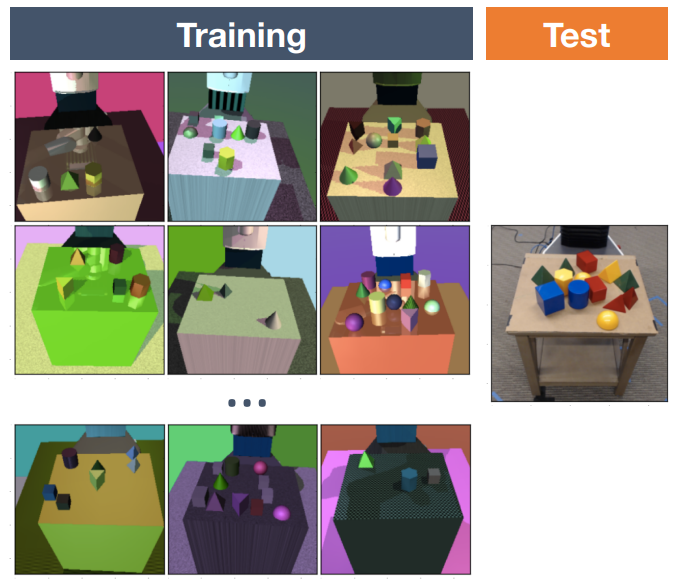
\includegraphics[width=\textwidth]{domain-randomization.png}
		\end{subfigure}
		\hfill
		\begin{subfigure}[b]{0.57\textwidth}
			\centering
			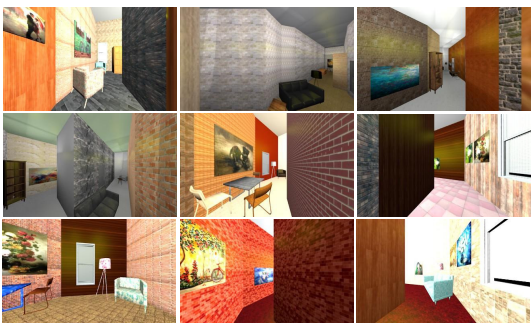
\includegraphics[width=\textwidth]{domain-randomization-1.png}
		\end{subfigure}
		\caption{Illustration of domain randomization \cite{sadeghi2016cad2rl, tobin2017domain}.}
		\label{fig:domain-randomization}
	\end{figure}	
	\item \citeausm{sadeghi2016cad2rl} randomize furniture, texture for drone's path planning problem.
\end{itemize}

\section{Adapting Simulation Randomization}
Domain randomization requires significant expertise and manual fine-tuning to design the distribution $ p(\xi) $ for simulation \ac{param}. In addition, overly wide distributions can hinder successful policy learning. The SimOpt approach adaptively optimize simulation \ac{param} with real-world experience. \cite{chebotar2019closing}

\section{Domain Adaptation}
\textit{Domain Adaptation} is the process that allow an \ac{AI} system trained in source domain to generalize to a target domain. In robotics, the source domain is the simulation and the target domain is the real world.
\begin{itemize}
	\item Labeled data is easily available from simulation / source domain
	\item Unlabeled data from real world / target domain can usually be collected, but labels are more difficult to obtain.
	\begin{itemize}
		\item \hlb{Unsupervised} domain adaptation: \hlr{no labels} in the target domain
		\item \hlb{Semi-supervised} domain adaptation: \hlr{fewer labels} in the target domain than in source domain
	\end{itemize}
	\item \textit{Pixel-level domain adaptation}: re-stylize images from the source domain to make them look like images from the target domain\\
	\note This is basically is neural style transfer in \ac{CV} with \ac{GAN}s\\
	Examples:
	\begin{itemize}
		\item \href{https://youtu.be/vDW8qvsBtmQ}{SimGAN} has \ac{GAN} and similarity loss \cite{shrivastava2017learning}
		\item \href{https://youtu.be/VhsTrWPvjcA}{PixelDA} adds task loss to the two above \cite{bousmalis2017unsupervised}
	\end{itemize}
	\item \textit{Feature-level domain adaptation}: focuses on learning domain-invariant features
	\begin{itemize}
		\item A mapping of fixed, pre-computed features between source and target domains \cite{sun2016return}
		\item DANN: A domain-invariant feature extractor with similarity loss (preferred method, using \ac{CNN}) \cite{ganin2016domain}
	\end{itemize}
\end{itemize}

Example:
\begin{itemize}
	\item Applying both pixel-level and feature-level domain adaptation: \citeaustitle{bousmalis2018using}
\end{itemize}

\section{Knowledge Distillation}
\textit{Policy distillation} is the process of extracting knowledge from a teacher network to a significantly smaller and more efficient student network, while maintaining a similarly expert level. The student is trained in a supervised manner with data generated by the teacher network.

\todo{DisCoRL, a modular, effective and scalable pipeline for continual learning}

\section{References}
\begin{itemize}
	\item Overview:
	\begin{itemize}
		\item \citeaustitle{hofer2020perspectives}
		\item \citeaustitle{zhao2020sim}
		\item Karol Arndt, Murtaza Hazara, Ali Ghadirzadeh, and Ville Kyrki. Meta reinforcement learning for sim-to-real domain adaptation. arXiv:1909.12906, 2019.
		\item Continual reinforcement learning deployed in real-life using policy distillation and sim2real transfer
	\end{itemize}
	\item Domain randomization:
	\begin{itemize}
		\item \citeaustitle{chebotar2019closing}
		\item \citeaustitle{tobin2017domain}
	\end{itemize}
	\item Domain adaptation:
	\begin{itemize}
		\item Pixel-level domain adaptation:
		\begin{itemize}
			\item \citeaustitle{shrivastava2017learning}
			\item \citeaustitle{bousmalis2017unsupervised}
		\end{itemize}
		\item Feature-level domain adaptation: \citeaustitle{ganin2016domain}
		\item Both: \citeaustitle{bousmalis2018using}
	\end{itemize}
	\item Knowledge distillation
\end{itemize}
	% !TeX spellcheck = en_US
\chapter{Natural Planning Model}
Structure is everywhere. An essay has a structure including the introduction, main body and conclusion. A house has a structure including the foundations, walls, roof. All living bodies, complex entities, organizations have structure. Within a structure, every part has its own responsibilities and connections with other parts. The clearer an entity is structured, the more functional and easier it is to improve. A body builder who wants to increase the size of his chest will go bench press, not squat. A company which wants to improve its branding will spend more investment on marketing, not logistics. As a roboticist, I asked myself: have robots follow a structured planning process (the answer is less or more). But the more challenging question is how could we bring more structure to robot planning? 

As always, it is beneficial to look at the robot's closest friend, the human kind. The rephrased questions would be: (1) do we think in structure? (2) is thinking with structure better than without it? (3) could we bring more structure to our thinking? For the first two questions, the answer is rather uncertain, as we are humans, but generally it is a "YES". \Eg, a good chess player will consider various aspects in a structured manner: hanging pieces, board space, king's safety, \etc. Experienced Sudoku solver will strategically scan over each number, each line, each row, each block. This also makes sense from the point of biology, specifically neuroscience. Our brains and the animals' brains are hierarchically structured. The animal's brain is structured into the forebrain, midbrain, hindbrain and spinal cord, in which the closer to the spinal cord, the more basic the functionalities a part is responsible for. Our brain is structured into the cerebrum, thalamus, brainstem and cerebellum. Studies have shown that there is clear difference in task complexity which each part is responsible for. \Eg: the cerebrum is responsible for high-level thinking, information processing (personality, decision-making, emotion, senses, language, \etc), while the cerebellum or brainstem are responsible for more basic muscle control and involuntary body functions (muscle memory, breathing, circulation, digestion, \etc)

The last and only question left is how to bring more structure into human thinking and robot planning? Whenever I come across ideas or approaches in other fields, I always try to find out whether there is possible connection or adaptation to robotics. I came upon this idea of the \textit{Natural Planning Model} which has various correspondences in robotics. The Natural Planning Model hypothesizes that the human brain tends to follow a five-step procedure before carrying on a sequence of complex actions \cite{allen2002getting}. 
\begin{enumerate}
	\item Defining Purpose and Principles
	\item Outcome Visioning
	\item Brainstorming
	\item Organizing
	\item Identifying Next Actions
\end{enumerate}

I would argue that we would manage to fit most of conducted robotic experiments in this 5-stage planning framework. That is because experiments are designed by humans, and that we unconsciously follow this natural planning model. Thus, the planning model is imprinted in their programs and the design of their experiments. The following parts cover the above steps and their corresponding robotic frameworks. I wish this framework to be the skeleton for other tools and modules, like the muscles, to attach to. If there are any current limitations (reaction time, accuracy, \etc), they should be limitations that can be tackled by improving other modules.

\section{Robot Planning}
Let's first have a definition of what does robot planning even mean. \cite{mcdermott1992robot, siciliano2008springer}
\begin{itemize}
	\item Robot planning is the \hlb{automatic generation, debugging, or optimization} of robot plans (or robot programs), by reasoning \hlr{explicitly} about the consequences of alternative plans.
	\item The plan needs not to be executed in its entirety. It should be the high-level plan, not low-level physical control. In addition, there can be changes that the plan needs to adapt, \eg chess.
	\item Purposes of a plan:
	\begin{itemize}
		\item keeps a certain state true,
		\item devise the most efficient plan for a certain task,
		\item react to a type of recurring world state,
		\item or some combination of all these things.
	\end{itemize}
	\item Ideally… the robot executes the plan while the planner thinks about improving it…	
\end{itemize}

\section{Purpose and Principles}
Purposes are the great answers to the "WHY" questions. We eat and drink to survive. We go to college in search for knowledge and skills. We travel and go out with our friends to relax and enjoy our lives. Well, for know, the simple yet sufficient "WHY" for robots is the fact that we, humans, are lazy and want our lives to be more comfortable :)

Principles are stated as the values that we hold for ourselves. These values create boundaries between the actions that are acceptable and those which are not. \Eg, those who treasure honesty would not lie to gain benefit. In similar manner, robots' principles would be the constraints that they have to operate under. If it's necessary, they will override lower-level commands. With that notion in mind, some of the basic constraints are:
\begin{itemize}
	\item Asimov's three law of robotics \cite{asimov2004robot}
	\begin{itemize}
		\item First Law: A robot may not injure a human being or, through inaction, allow a human being to come to harm.
		\item Second Law: A robot must obey the orders given it by human beings except where such orders would conflict with the First Law.
		\item Third Law: A robot must protect its own existence as long as such protection does not conflict with the First or Second Law.
	\end{itemize}
	\item Other safety and physical constraints, in terms of force, torque, velocity, acceleration
	\item Task-related constraints: \eg, in chess, there are rules about how a piece moves
\end{itemize}

\section{Outcome Visioning}
Knowing the answer to the "WHY" question, we start envision the desired outcomes, the answers for the "WHAT" questions. A chef imagines what food is on the final plate, how they taste, look and smell like. An architect imagines what rooms, functionalities a house has, how each room looks like, how the light, air, water travel in the house.

Some robotic works have followed this line of thought:
\begin{itemize}
	\item Goal-conditioned learning
	\begin{itemize}		
		\item \todo{cite goal-proposed RL exploration mechanism}
		\item \citeaustitle{andrychowicz2017hindsight}
	\end{itemize}
	\item Contextual learning \todo{}
	\item Multi-model goal "imagination"
	\begin{itemize}
		\item \citeaustitle{sharma2019third} (badly written, but still)
		\item \todo{}
	\end{itemize}
\end{itemize}

\section{Brain Storming and Organizing}
Brain Storming and Organizing are two separate steps. Brainstorming is the step in which we start breaking down the desired goal in an unstructured way. We list out related entities (relevant subtasks, objects, people) in an unordered manner. For example, with the goal to have a dinner with friends, following problems could arise in one's mind in unordered sequence: are our friends available, where would we eat, what time will we meet, do they have specific allergies. Then, organizing is the step when we start putting these subtasks, other entities into relations and sequence based on prioritization. For the prior example, we start with creating a group chat to discuss (check availability, date and time), then we call the restaurant (check availability, book table).

Existing robotic frameworks can be divided into two problems:
\begin{itemize}
	\item Interpreting the interaction, relation with other entities (objects, agents)
	\item Breaking down a complex task into sequence of simple known tasks
\end{itemize}

\subsection{Interaction Planning}
\begin{itemize}
	\item Interaction with other objects using a graph, in which the nodes are objects and the robot itself
	\begin{itemize}
		\item \citeaustitle{lin2022efficient}
		\item \citeaustitle{sieb2020graph}
	\end{itemize}
	\item Relation with other agents / robots
	\begin{itemize}
		\item \citeaustitle{zhang2019robot}
	\end{itemize}
\end{itemize}

\subsection{Breaking Down the Plan}
\begin{itemize}
	\item Explicit planning by human
	\begin{itemize}
		\item \citeaustitle{smith2019avid}
		\item \citeaustitle{brooks1982symbolic}		
	\end{itemize}
	\item Learning and formalizing a plan with symbolic representation and action grammar.
	\begin{itemize}
		\item \citeaustitle{zhang2019robot}
		\item \citeaustitle{toussaint2018differentiable}				
		\item \citeaustitle{yang2015robot}
	\end{itemize}
\end{itemize}

Sometimes, there are many possible plans to reach a goal. Then plan could be chosen based on addition constraints or rules for optimization / selection. \Eg, to cook a dish with a piece of steak, potatoes and veges, one could vary on the ingredient to start with, and switch to work on the others any time. The time duration to finish cooking, the quality of the food could be included as additional constraints to cancel out redundant plans.

\section{Identifying and Taking Action}
A library of primitive actions plays a great role. A primitive action should be meaningful, but also general enough to be efficient. Some works focus on motor control (force and torque) that leads to jiggering motion artifacts. We don't want the arm to move around like that. We want a smooth and decisive movement, but of course, can still subject to minor error and stochasticity.

Generality implies that if we want to go to 1 from 0, we don't want to step by step specify it to go to 0.1, 0.2, \etc. What we want is for it to go to the neighbor of 1 in one single movement.

\begin{itemize}
	\item Motor primitives \cite{ijspeert2002movement}
	\item \todo{}
\end{itemize}

Goal-based policy learning
\begin{itemize}
	\item 
\end{itemize}

\section{References}
\todo{}
\begin{itemize}
	\item Robot planning
	\begin{itemize}
		\item \note A great but long and complex paper: \citeaustitle{mcdermott1992robot}
		\item \citeaustitle{brooks1982symbolic}
	\end{itemize}
	\item Goal imagining mechanism: wide range of works
	\item Goal-conditioned learning:
	\item Learning action plan
	\item Primitive motion
\end{itemize}
	% !TeX spellcheck = en_US
\chapter{Research Proposal}

\section{Introduction and Background of Interest}

\todo{ignore for now}

Robots are complex machines designed to support our lives.

Since mid 19th century, its emergence has received research attention in both the academic and industry. The first major application was in the automotive industry. Its presence is entering our lives in different fields is spreading even more and more. \todo{move to unstructured environments and challenges}

\section{Literature Review}

To my best current knowledge, robot arms have made significant improvement, but are still far from delivering general-purpose tasks. Initially, robot arms are programmed explicitly and only capable of working in the known and constrained environment of factories. Progress in different fields of technology has provided the robots more inputs (\eg, vision, audio, haptic) to operate in dynamic and unstructured environments. State-of-the-art robot manipulators can deliver complex tasks, \eg, cooking \cite{moley}, making coffee \cite{coffeemaster}, and cleaning around the house \cite{bothandy}. However, the behaviors of these models are still awkwardly disruptive and far from the mastery level of the human hand's dexterity. In addition, instead of having the adaptability for a wide range of conditions, most models still operate in designed environments with known tools and settings.

\subsection{Robotic Grasping}

Grasping is one of the critical and unavoidable problems for robot manipulators, especially for logistic and service robots. Overall, most successful grasping approaches are empirical, using deep learning on a large dataset to find the best grasping candidates. Majority of models are supervised learning using single-modal input, \ie RGB images. A few have considered multi-modal inputs: RGB with depth images or tactile input. Approaches, which take tactile data, use it as the sole input to improve grasp stability, adaptability to object's weight \cite{bekiroglu2011assessing, li2014learning}, a few combine with other modality for improvement \cite{calandra2017feeling}. \cite{bohg2013data, caldera2018review, li2019review, kleeberger2020survey}

\subsection{Reinforcement Learning}
\ac{RL} is a branch of \ac{ML} approaches for learning decision making from experiences. Given a sufficient amount of input data, it can potentially surpass human's ability for reasoning, \eg, playing games like Go, chess, Atari. Most works on robot manipulators are currently directed to object picking and hand-over tasks. To meet the need for data, sim-to-real transfer techniques \cite{kleeberger2020survey} and collective learning are being studied \cite{yahya2017collective}. Unlike in other domains of \ac{ML}, it's difficult to implement transfer learning with \ac{RL}, given different robot arms, gripper and sensor types. Various directions are being researched to tackle this issue, \ie offline \ac{RL}, novel exploration strategies, multi-task learning, meta-learning. \cite{kober2013reinforcement, li2017deep, arulkumaran2017deep, singh2021reinforcement}

\section{Approaches and Choice of Methods}
\subsection{Key Points for Improvement}
Prior works on robotic manipulators were limited on their utilization of tactile sensors. Because complex hand and arm behaviors need force and pressure feedback, leveraging the manipulators to the dexterity level of human's arms requires these sensors. However, tactile sensors are currently been used mostly for the development of soft robotics \cite{haddadin2018tactile}. For grasping tasks, despite certain successes from using visual and tactile input separately, there hasn't being a multi-modal approach capable of combining the strengths of both sides, \ie, accurate localization, adaptability to object properties. A model, which has knowledge from both visual and tactile sources, promises to deliver complex manipulation tasks with diverse objects.

It's still challenging to generalize and apply \ac{RL} to different robotic manipulator's tasks. In general, \ac{RL} did make a convincing case about its potential to surpass human's ability in some specific applications, \eg, playing Go, chess. However, in other fields, practical applications are yet scattered and limited. For robotic manipulators, current focuses are still around object picking and handling tasks \cite{singh2021reinforcement}. One of the major causes for this situation is the current gap in generalization and transfer learning. Directions for improvements are meta-learning, multi-task learning, \etc \cite{kober2013reinforcement}.

\subsection{Approaches and Research Contributions}
The progress I wish to work towards concerns robotic collective learning for collaborative tasks. For example, a system of multiple robot arms learning to play 2v2 table tennis, pack an item or cook. Building up towards this progress, I intend to work and gain more experiences on the following problems:

\begin{enumerate}
	\item A multi-modal approach for robotic picking task: combines visual and tactile input into a \ac{DL} model. Prior works on tactile sensors have proven their potentials in inference of object properties \cite{luo2017robotic} and improving robotic grasping \cite{yamaguchi2019recent}. I want to further extend recent advances in tactile sensors to a multi-modal approach.
	\item Visual imitation learning: copies behaviors from visual demonstrations (videos). Prior works are still restricted with certain types of input data, tasks \cite{finn2017one, sharma2019third}. 	Based on previous progress on teleoperation \cite{handa2020dexpilot}, I want to extend further to learn in different problem settings, with generalized tasks, and also apply offline \ac{RL}.
	\item A data collection pipeline for robot manipulators: preferably from using the above visual imitation learning, to map human’s arm movements to manipulator's. The data would contain both visual and tactile information. It would then be used for the learning of other robotic tasks or in other settings (different types of arm, gripper, \etc).
	\item Meta-learning with different manipulation tasks.
\end{enumerate}

Moreover, I'm also interested in exploring the usage of certain \ac{DL} models, techniques:
\begin{itemize}
	\item Generative model: Generating expert-like samples.
	\item Score matching
	\item Exploration for imitation learning
\end{itemize}

\section{Proposed Research Plan}

\todo{}

\todo{How the lab is related to this research plan?}
\begin{itemize}
	\item There is alignment in our directions
	\item Fit the position
\end{itemize}

\todo{Give compliments to their works!}
\begin{itemize}
	\item mention more explicitly regarding the topics, what research they have done
	\item I read your papers about … let alone the works on …
\end{itemize}

	% !TeX spellcheck = en_US
\chapter{Technical Tools}

This chapter talks about or at least lists out helpful tools, platforms for using/working with robotics.

\section{MuJoCo}
\begin{itemize}
	\item \href{https://youtu.be/Fiq_hpaoeH0}{MuJoCoPy Lec 2a: 2D Manipulator modeling (Part 1 of 2)}
\end{itemize}

\section{ROS}
\begin{itemize}
	\item \href{https://youtube.com/playlist?list=PLE-BQwvVGf8HOvwXPgtDfWoxd4Cc6ghiP}{Programming for Robotics (ROS)}
\end{itemize}

	
	\backmatter
	\pagenumbering{Roman}
	\printbibliography[heading=bibintoc]
	\appendix
\end{document}